\documentclass[a4paper]{report}

\usepackage[utf8]{inputenc}
\usepackage[T1]{fontenc}
\usepackage[french]{babel}
\usepackage{amsmath}
\usepackage{graphicx}
\usepackage{numprint}
\usepackage{enumitem}
\usepackage{scrextend}
\usepackage{a4wide}
\usepackage{float}
\usepackage{textcomp, gensymb}
\usepackage{booktabs}
\usepackage{array}
\usepackage{tabularx}
\usepackage{minted}
\usepackage{algpseudocode}
\usepackage[toc,page]{appendix}
\usepackage[final]{pdfpages}
\usepackage[footnote]{acronym}
\usepackage[export]{adjustbox}
\usepackage[lofdepth,lotdepth]{subfig}
\usepackage{hyperref}
\usepackage[colorinlistoftodos]{todonotes}

\renewcommand{\labelenumii}{\theenumii}
\renewcommand{\theenumii}{\theenumi.\arabic{enumii}.}

\let\EndItemize\enditemize
\def\enditemize{\EndItemize\bigskip}

\newenvironment{absolutelynopagebreak}
  {\par\nobreak\vfil\penalty0\vfilneg
   \vtop\bgroup}
  {\par\xdef\tpd{\the\prevdepth}\egroup
   \prevdepth=\tpd}

\setlength{\parindent}{2em}
\setlength{\parskip}{1em}
\addtokomafont{labelinglabel}{\bf}

\begin{document}

%%%%%%%%%%%%%%%%%%
%%% First page %%%
%%%%%%%%%%%%%%%%%%

\begin{titlepage}
\begin{center}


\includegraphics[width=0.6\textwidth]{img/logo_polytech.png}\\[1cm]

{\large Informatique Industrielle en apprentissage}\\[0.5cm]

{\large Projet de Fin d'Étude}\\[0.5cm]

% Title
\rule{\linewidth}{0.5mm} \\[0.4cm]
{ \huge \bfseries Or-Box - Analyse \& modélisation \\[0.4cm] }
\rule{\linewidth}{0.5mm} \\[1.5cm]

% Author and supervisor
\noindent
\begin{minipage}{0.4\textwidth}
  \begin{flushleft} \large
    \emph{Auteur :}\\
    M.~Pierre \textsc{Robillard}\\
  \end{flushleft}
\end{minipage}%
\begin{minipage}{0.4\textwidth}
  \begin{flushright} \large
    \emph{Encadrant :} \\
    M.~Frédéric \textsc{Rayar}\\
  \end{flushright}
\end{minipage}

\vfill

% Bottom of the page
{\large Version 0.1 du\\ \today}

\end{center}
\end{titlepage}

\tableofcontents
\listoffigures

\chapter*{Liste des sigles et acronymes}
\begin{acronym}[HATEAOS] % Give the longest acronym here

\acro{CEM}{Compabilité Électro-Magnétique}
\acro{COTS}{\emph{Component Off the Shelf}}
\acro{CMS}{Composant Monté Surface}
\acro{CRUD}{\emph{Create Read Update Delete}}
\acro{DAC}{\emph{Digital to Analog Converter}}
\acro{DII}{Département Informatique Industrielle}
\acro{HATEAOS}{\emph{Hypermedia As The Engine Of Application State}}
\acro{MOA}{Maître (\emph{ou Maîtrise}) d'Ouvrage}
\acro{MOE}{Maître (\emph{ou Maîtrise}) d'\OE{}uvre}
\acro{PCB}{\emph{Printend Circuit Board}}
\acro{PWM}{\emph{Pulse Width Modulation}}
\acro{PFE}{Projet de Fin d'étude}
\acro{REST}{\emph{REpresentational State Transfer}}
\acro{SVM}{\emph{Support Vector Machine}}
\acro{UX}{\emph{User Experience}}
\acro{V4L}{\emph{Video for Linux}}
\end{acronym}

\chapter{Porté du document}

    \section{Domaine d'application}
    
    Le domaine d’application se limite à la OrBox --- un PFE pour le département d'Informatique Industrielle de Polytech Tours.
    Pour rappel, la Or-Box est un système destiné aux personnes souffrant de déficience visuelle.
    Elle a pour but de les aider au quotidien à reconnaître et distinguer des objets de la vie courante, et ce malgré leur handicap.
    
    \section{Porté du document}
    
    L’objet du document est de décrire les modèles mis en place pour réaliser les différentes fonctions nécessaires au système ainsi que leur implémentation.
    Dans la première partie du document, un court rappel de l'architecture globale du système est effectué.
    Les implémentations techniques déjà réalisées à ce jour seront exposées dans le deuxième chapitre de ce document.
    La dernière partie du document fournit une description algorithmique détaillée des fonctions de \emph{computer vision}.
    
    Pour mémoire, les spécifications du système sont décrites dans \cite{OBCdS}, la lecture préalable de ce dernier est recommandée.
    

\chapter{Architecture globale}
% rappeler les différents blocks SysML identifié

Ce chapitre est une description succincte de la modélisation statique du système faite dans \cite{OBCdS}.
La figure \ref{TopBDD} ci-dessous montre l'architecture matérielle et logicielle du système global, elle suit le formalisme SysML.

\begin{figure}[H]
	\centerline{
		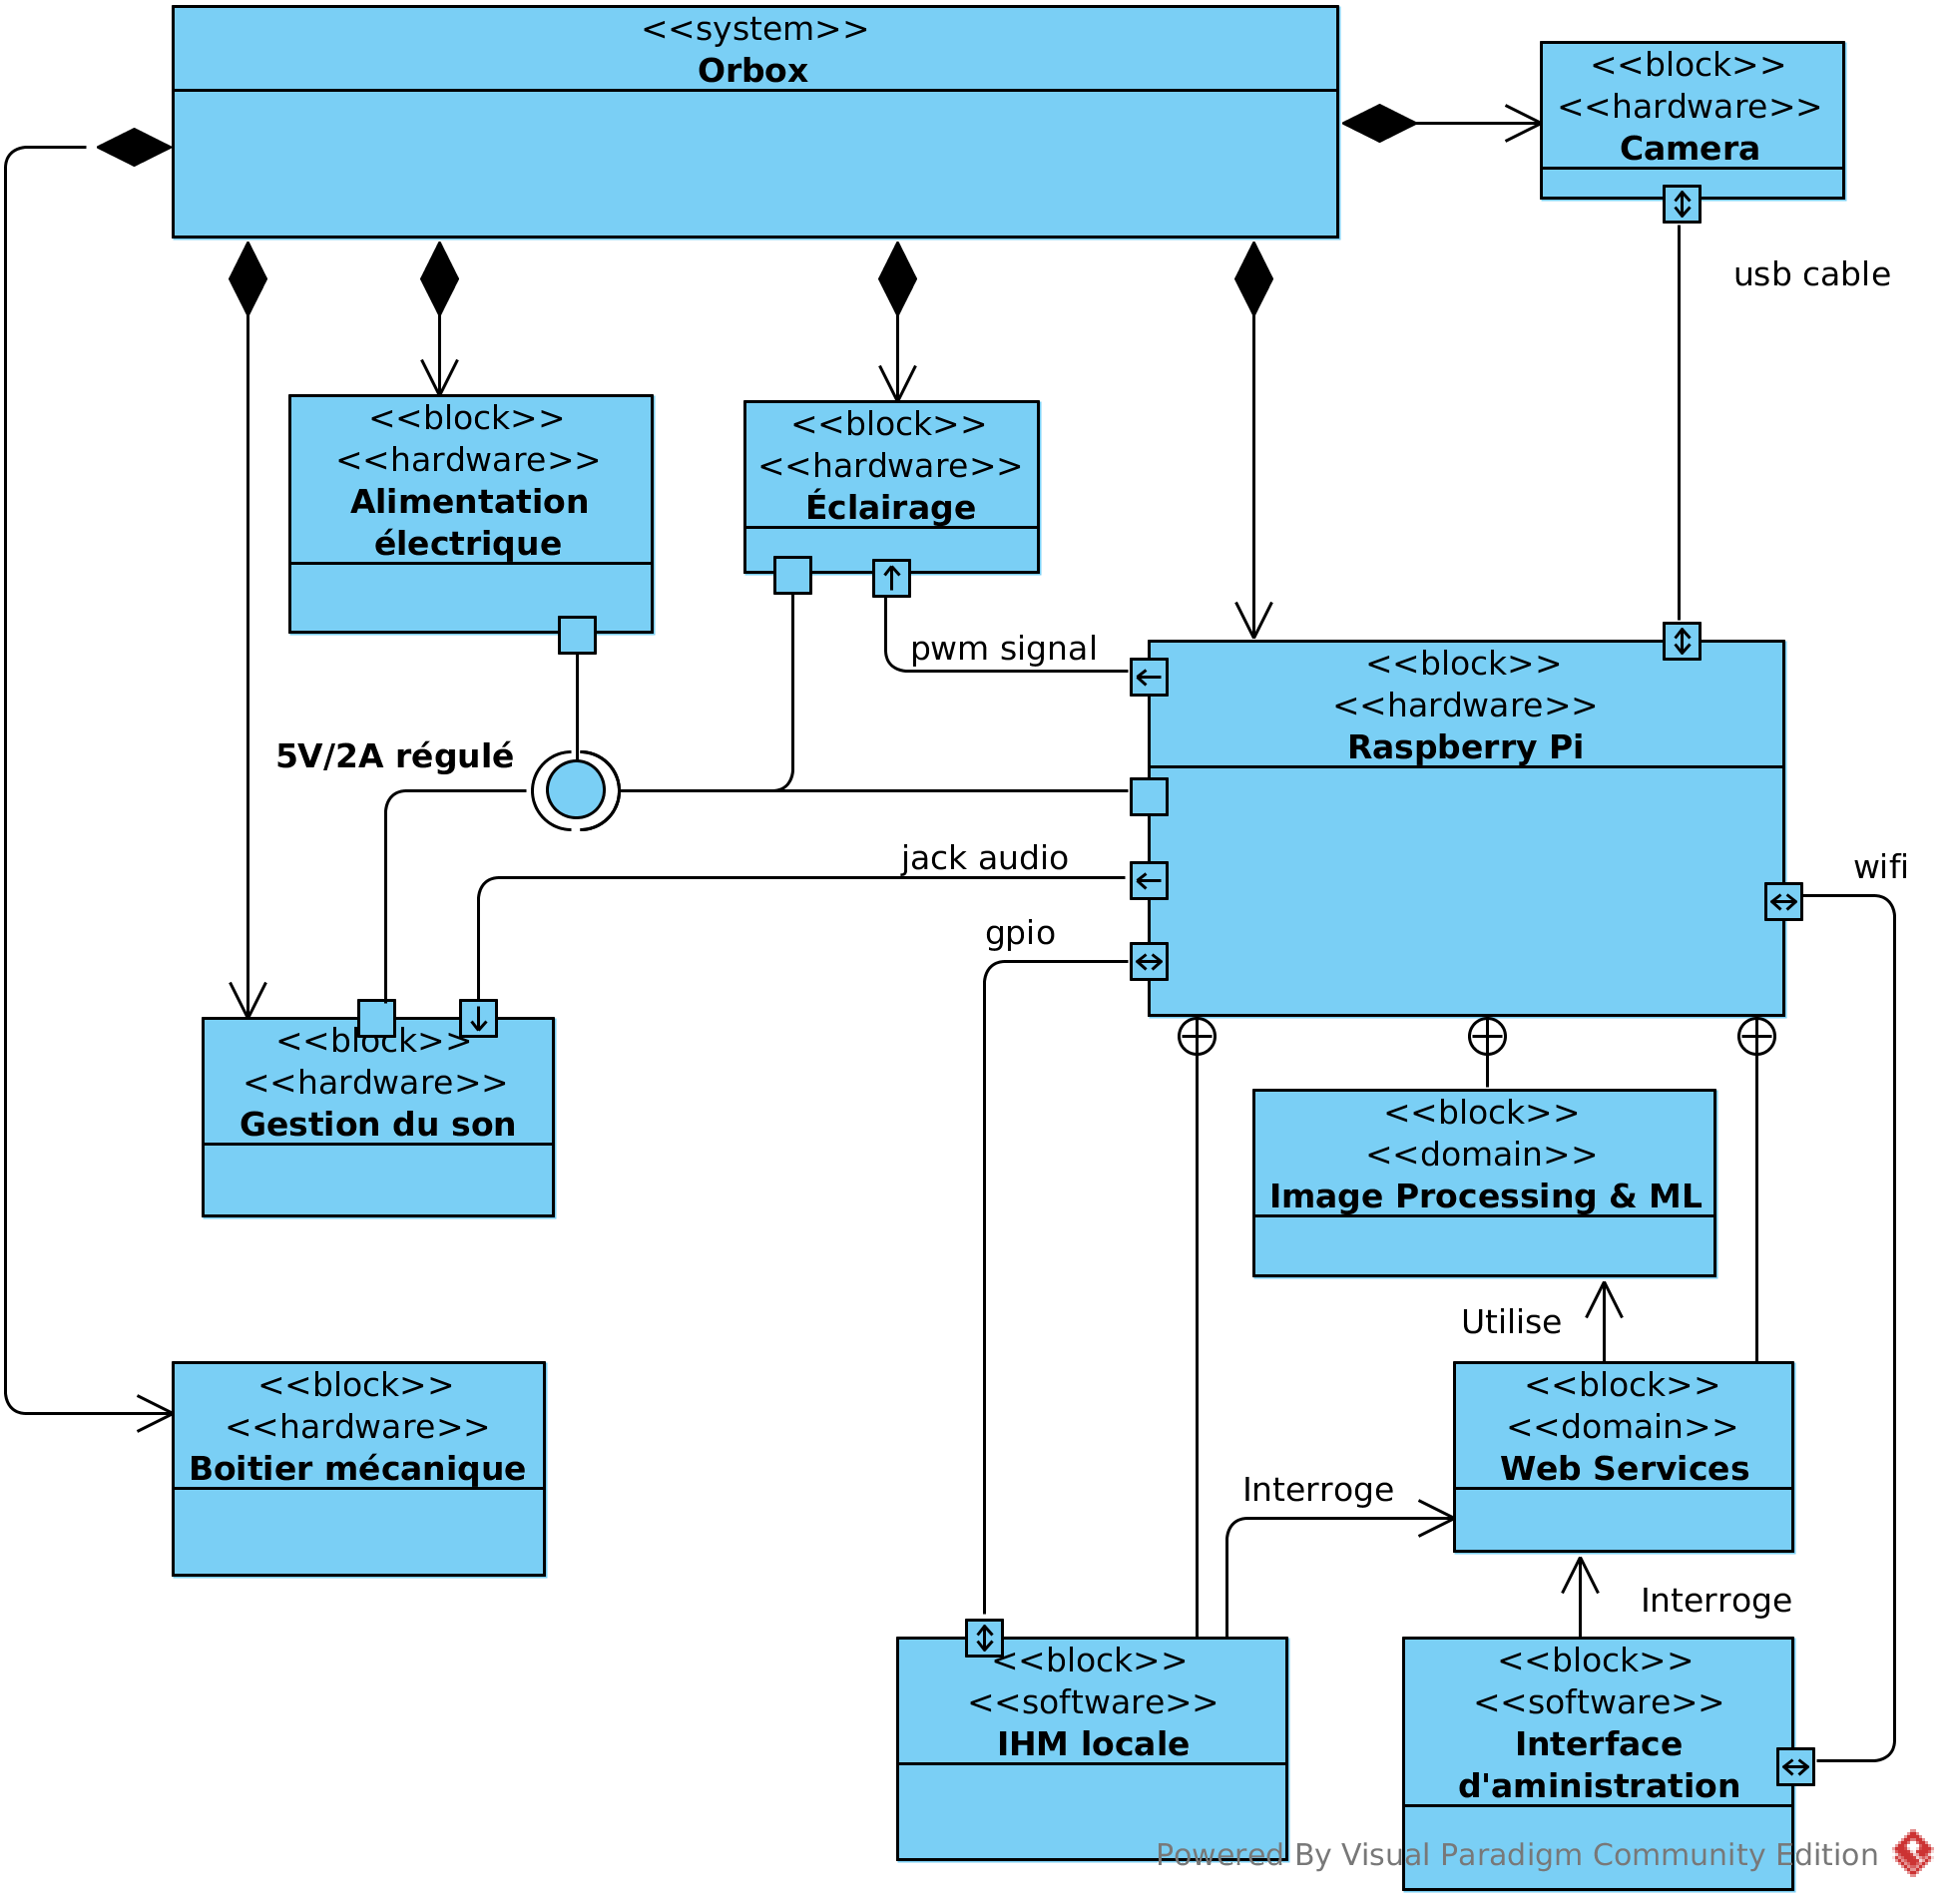
\includegraphics[scale=0.75,fbox]{img/SysML_Top_BDD.png}
	}
	\caption{Top level Block Definition Diagram}
	\label{TopBDD}
\end{figure}

Une description détaillée des composants est fournie ci-dessous :
\begin{labeling}[~--]{Interface d'administration}
	\item [Alimentation électrique] Elle a pour rôle de fournir l'énergie de manière suffisante et appropriée aux composants électroniques de la Or-Box.
	\item [Boitier mécanique] Il sert à maintenir les différents composants matériels ensemble.
	\item [Gestion du son] Elle permet de transformer et d'adapter le signal électrique en signal sonore pour la synthèse vocale.
	\item [Éclairage] Il permet d'avoir des clichés des objets posés sur la vitre malgré le contre-jour créé par la lumière ambiante.
	\item [Caméra] Elle est équipée d'un objectif fish-eye de 170 \degree d'angle de vue afin de voir toute la surface vitrée tout en maintenant un design compact.
	\item [Raspberry Pi] C'est l'ordinateur monocarte embarqué dans le système sur lequel est exécute l'ensemble des composants logiciels.
	\item [Interface d'administration] Application déportée de la Or-Box qui permet d'enrichir la base d'objet connu.
	\item [IHM Locale] Le composant logiciel qui a pour but d'orchestrer les scénarios de la Or-Box quand elle utilisé de manière autonome.
	\item [Web Services] Ils permettent l'accès à des ressources qui devront être accédées par l'interface distante d'administration et par l'IHM locale.
	\item [Image Processing \& ML]  Ce bloc logiciel contient le coeur de métier de l'application, voir le chapitre \ref{AnaLog} pour plus de détails.
\end{labeling}



\chapter{Réalisation}
    \section{Électronique}
    % mettre analyse SysML et Schéma électronique cote à cote
    
    Le schéma structurel et le routage de la carte ont été effectués avec le logiciel en ligne UpVerter\footnote{Schéma : \href{https://upverter.com/OrboxTeam/cfa40d292bac9e7b/Orbox_PFE/}{OrBox PFE - upverter.com} --- Nomenclature : \href{https://docs.google.com/spreadsheets/d/1U8SqlsJ5GUVQXFXz04T_kTUTFbFambgKo4qdCGi8VkM/edit?usp=sharing}{BOM - docs.google.com}}. Cette section donne des précisions sur la manière dont chaque fonction électronique a été implémentée. 
        
\begin{figure}[H]
    \centerline{
        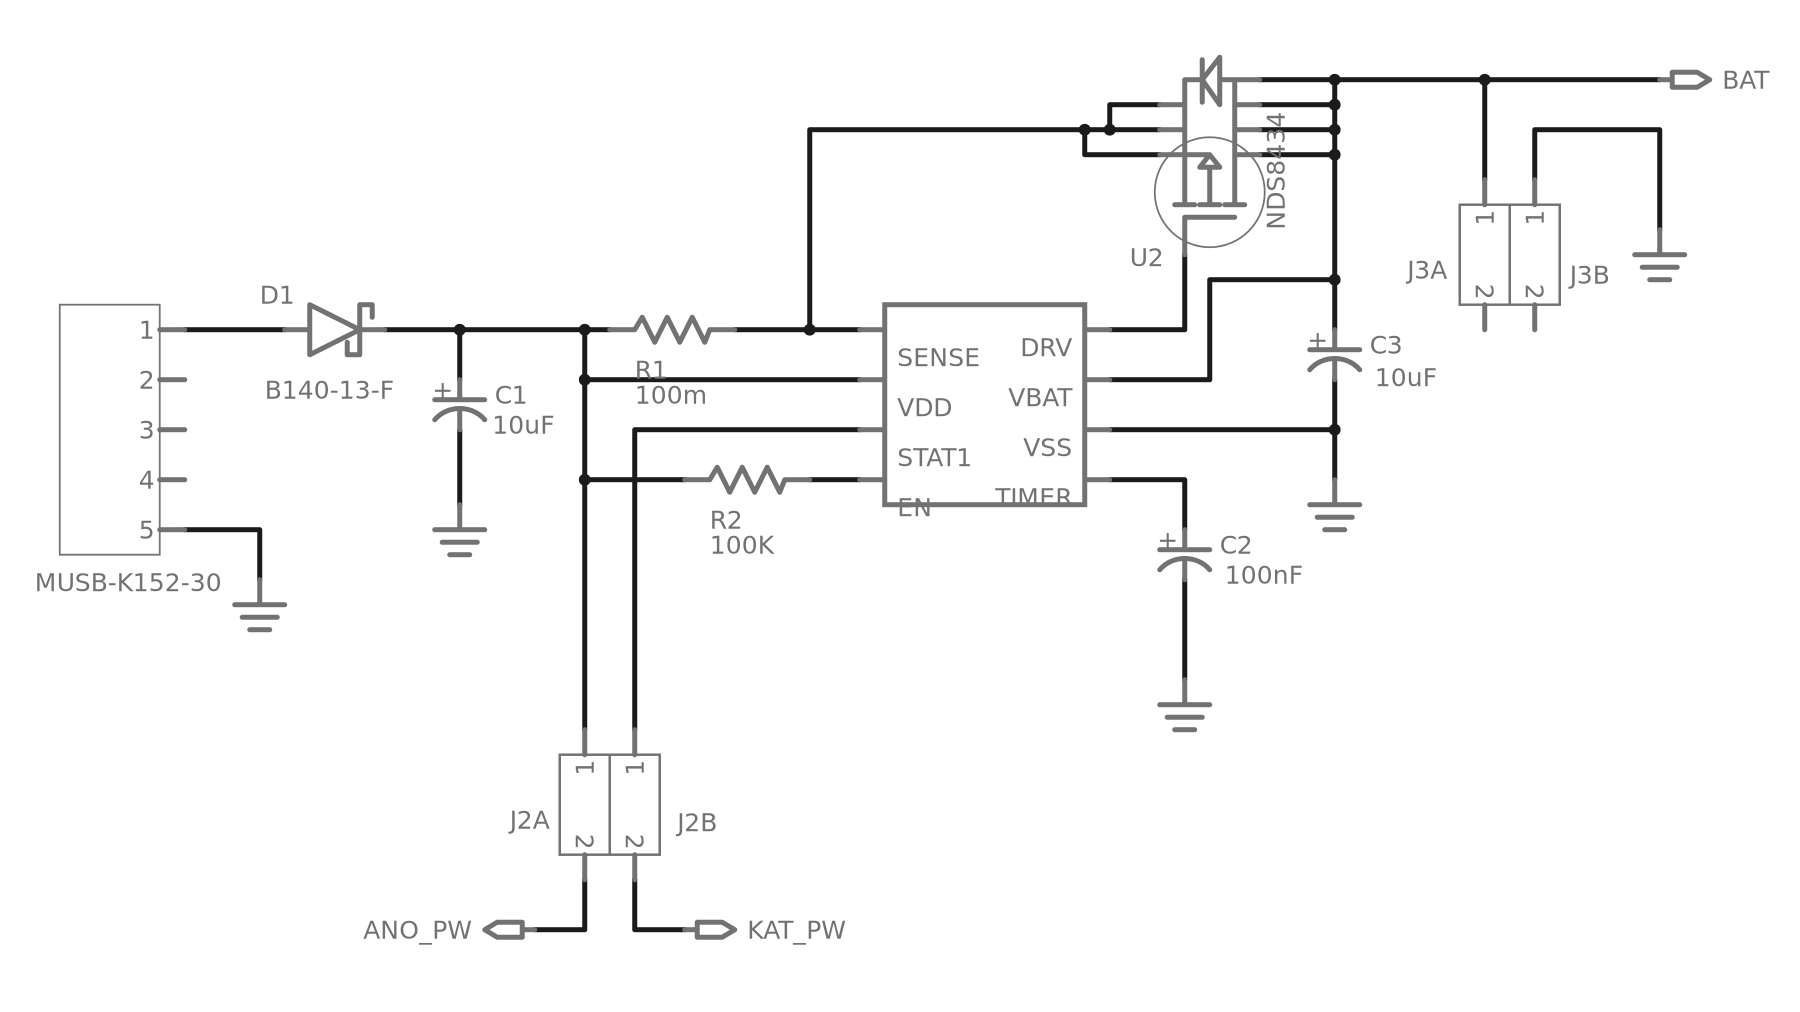
\includegraphics[width=0.85\textwidth,fbox]{img/ElecSch_BatCharger}
    }
    \caption{Schéma structurel du régulateur de charge}
    \label{ElecSch_BatCharger}
\end{figure}

    La fonction électronique \emph{régulateur de charge} est réalisée autour du composant MCP73843 (repère typographique $U_1$ de la Figure \ref{ElecSch_BatCharger}).
    Pour rappel, la fonction régulateur de charge a pour rôle de prendre la tension d'entrée de 5V délivrée par le chargeur USB mural pour l'abaisser à une tension acceptable pour la batterie Li-Ion Polymer comprise entre 3.7V et 4.2V.
    
    Le composant $J_1$ est un connecteur micro-AB USB 2.0 qui accepte aussi bien les prises micro-A que micro-B.
    Le MCP73843 permet de piloter la led d'indicateur de charge directement sans led, elle se branche au bornier $J_2$.
    La batterie sera quant à elle branchée au bornier $J_3$.
    Le dimensionnement des composants annexes suit les recommandations du fabricant pour un usage nominal.

\begin{figure}[H]
    \centerline{
        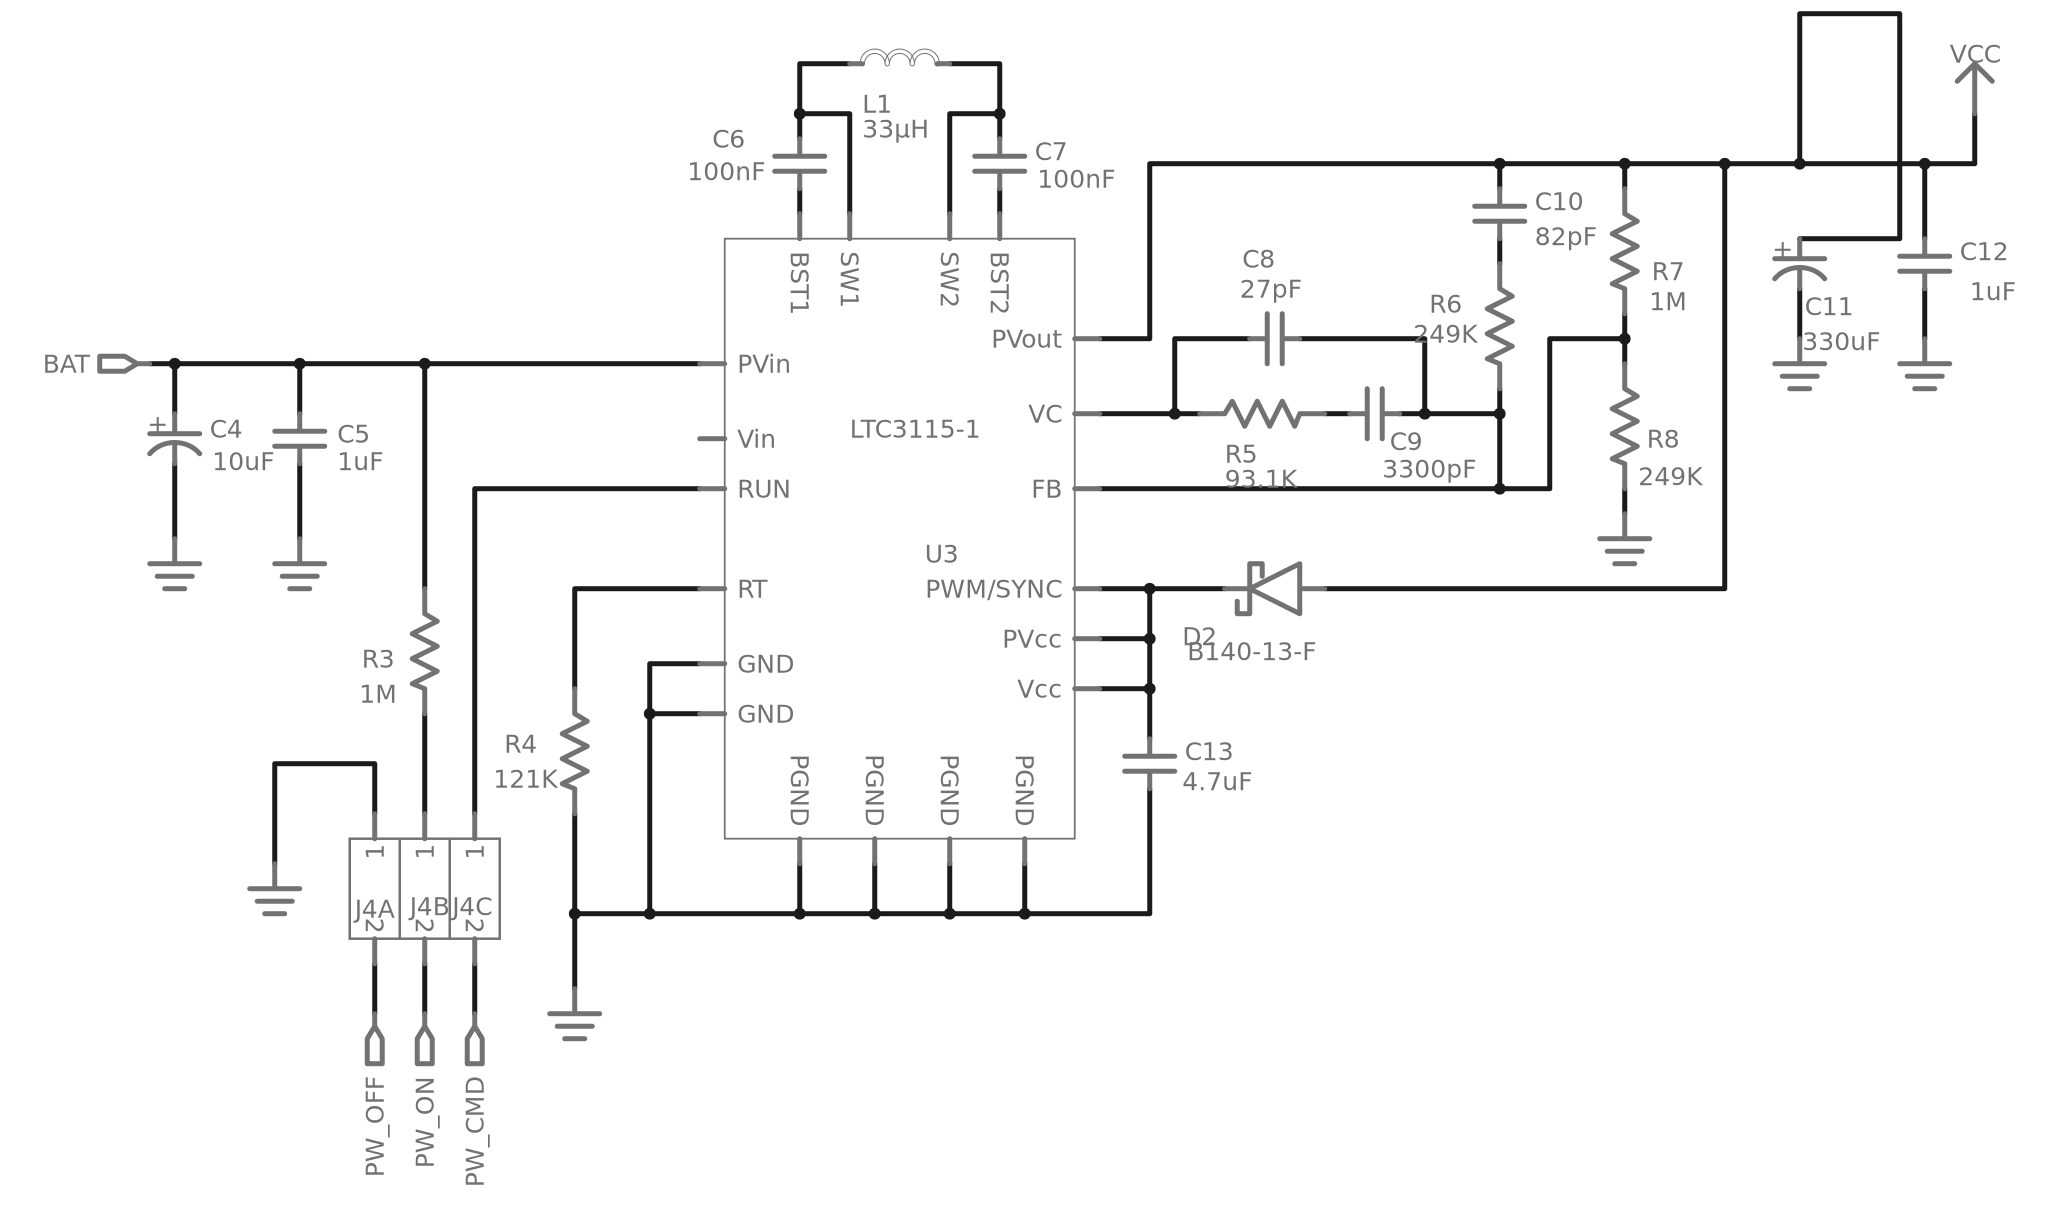
\includegraphics[width=0.85\textwidth,fbox]{img/ElecSch_BuckBoost}
    }
    \caption{Schéma structurel du régulateur de tension}
    \label{ElecSch_BuckBoost}
\end{figure}

    La fonction électronique \emph{régulateur de tension} est réalisée autour du composant LTC3115-1 (repère typographique $U_3$ de la Figure \ref{ElecSch_BuckBoost}).
    Pour rappel, la fonction régulateur de tension a pour rôle de prendre la tension délivrée par la batterie qui varie entre 3.7V et 4.2V suivant sa charge et de la convertir en 5V stabilisé afin d'alimenter le Raspberry Pi, l'amplificateur audio et le driver de led.
    Ce convertisseur de tension est une alimentation à découpage de type Buck-Boost.
    
    La boucle de retour est un filtre du troisième ordre dont la fonction de transfert :
    
    \todo[inline]{TODO}

\begin{figure}[H]
    \centerline{
        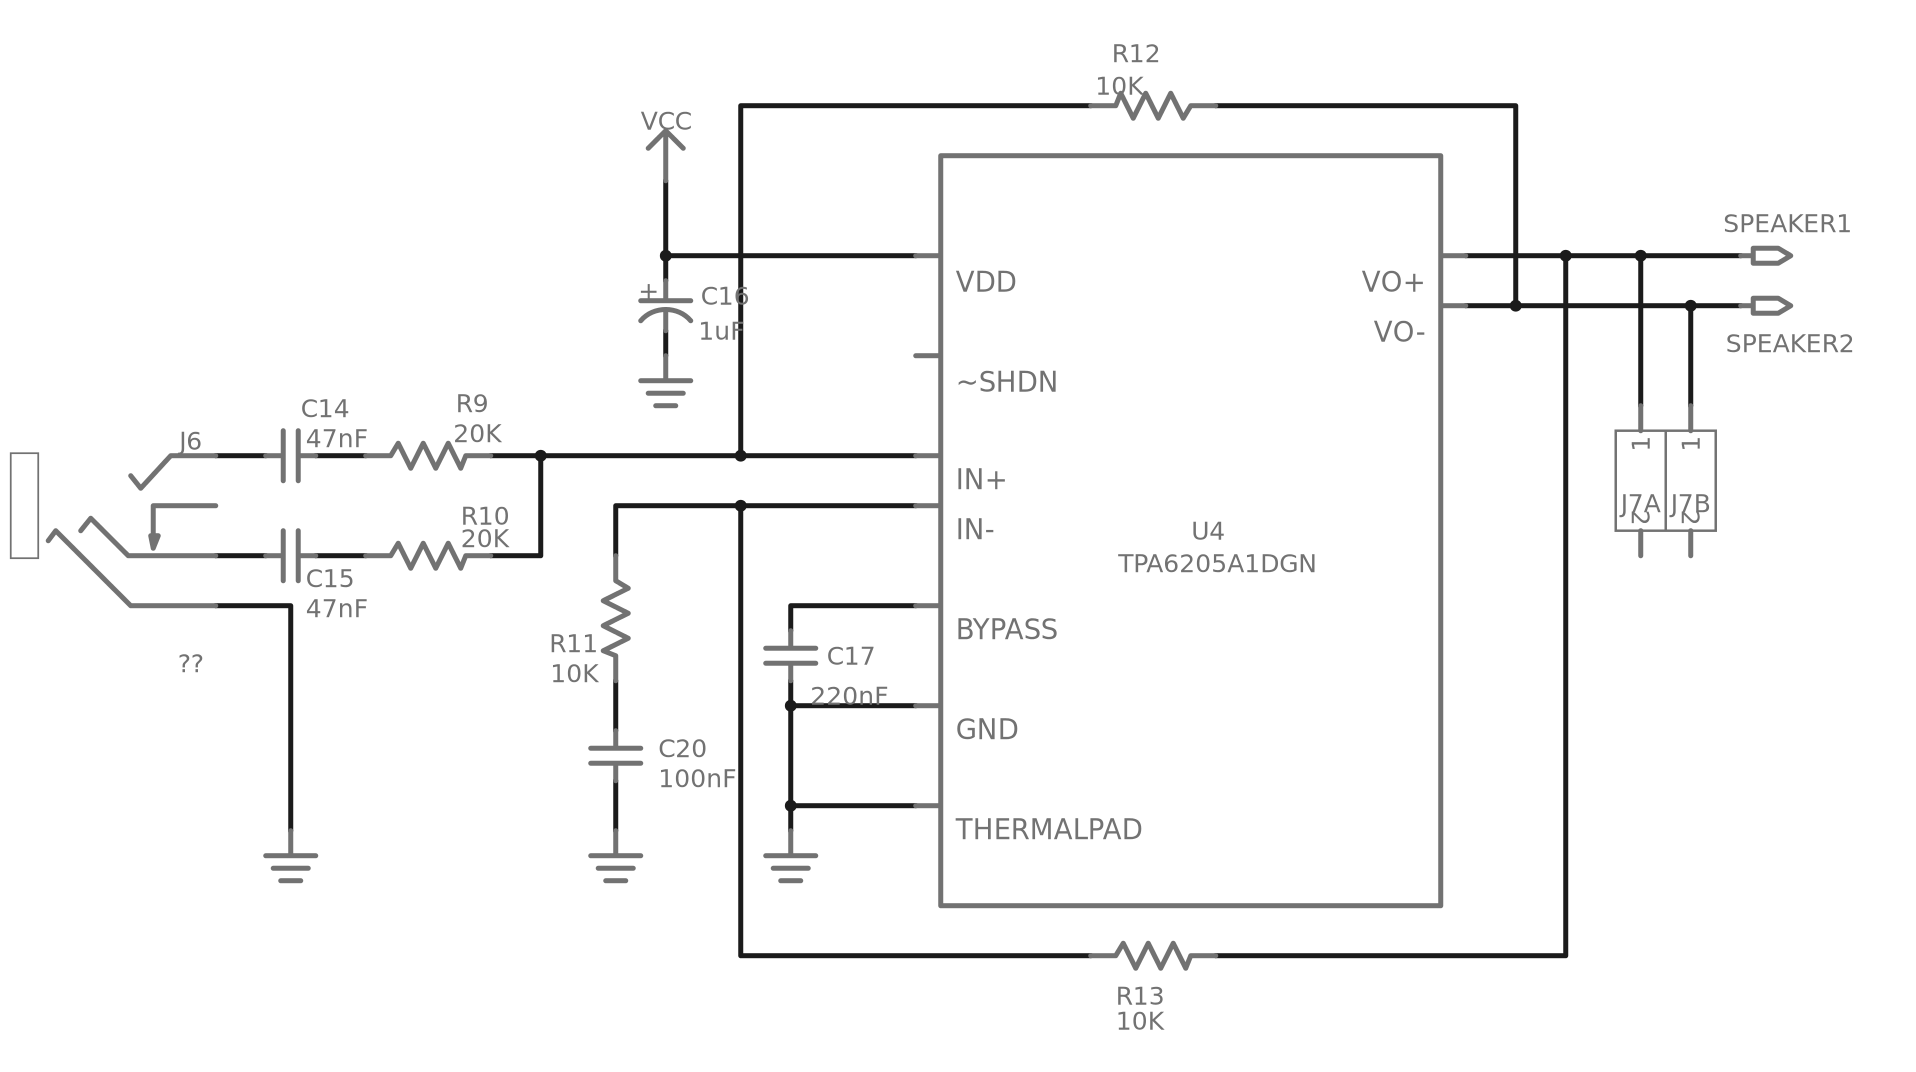
\includegraphics[width=0.85\textwidth,fbox]{img/ElecSch_AudioAmp}
    }
    \caption{Schéma structurel de l'amplificateur audio}
    \label{ElecSch_AudioAmp}
\end{figure}

    La fonction électronique \emph{amplificateur audio} est réalisée autour du composant TPA6205A1DGN (repère typographique $U_4$ de la Figure \ref{ElecSch_AudioAmp}).
    Pour rappel, la fonction amplificateur audio a pour rôle de récupérer le signal audio stéréo de synthèse vocale généré par le Raspberry Pi disponible sur le connecteur jack 3.5 mm, de sommer les deux voies et d'amplifier le signal afin d'attaquer le haut-parleur de 8 $\Omega$ relié au bornier $J_7$.
    
    Les deux condensateurs $C_{14}$ \& $C_{15}$ sont des condensateurs de liaison permettant d'enlever la composante continue de chaque voie.
    Les impédances de chaque entrée différentielle de l'amplificateur doivent être équilibrées, pour cela il faut respecter les relations suivantes :
    
\begin{subequations}
\begin{align}
C20 &= C15 + C14 \\
100nF &\approx 47 nF + 47 nF
\end{align}
\end{subequations}
\begin{subequations}
\begin{align}
R_{11} &= \frac{R_9 \times R_{10}}{R_9 + R_{10}}\\
10 k\Omega &= \frac{(20 k\Omega)^{2}}{2 \times 20 k\Omega}
\end{align}
\end{subequations}
    
    Le gain d'amplification et la fréquence de coupure pour chaque voix est :
    
\begin{equation}
Gain = 20 \times log \left (\frac{2 \times 150 k\Omega}{R_9}\right ) = 20 \times log \left (\frac{2 \times 150 k\Omega}{R_{10}}\right ) \approx 23.5 dB
\end{equation}
\begin{equation}
F_{C} = \frac{1}{2 \pi R_9 C_{14}} = \frac{1}{2 \pi R_{10} C_{15}} = 169 Hz
\end{equation}

\begin{figure}[H]
    \centerline{
        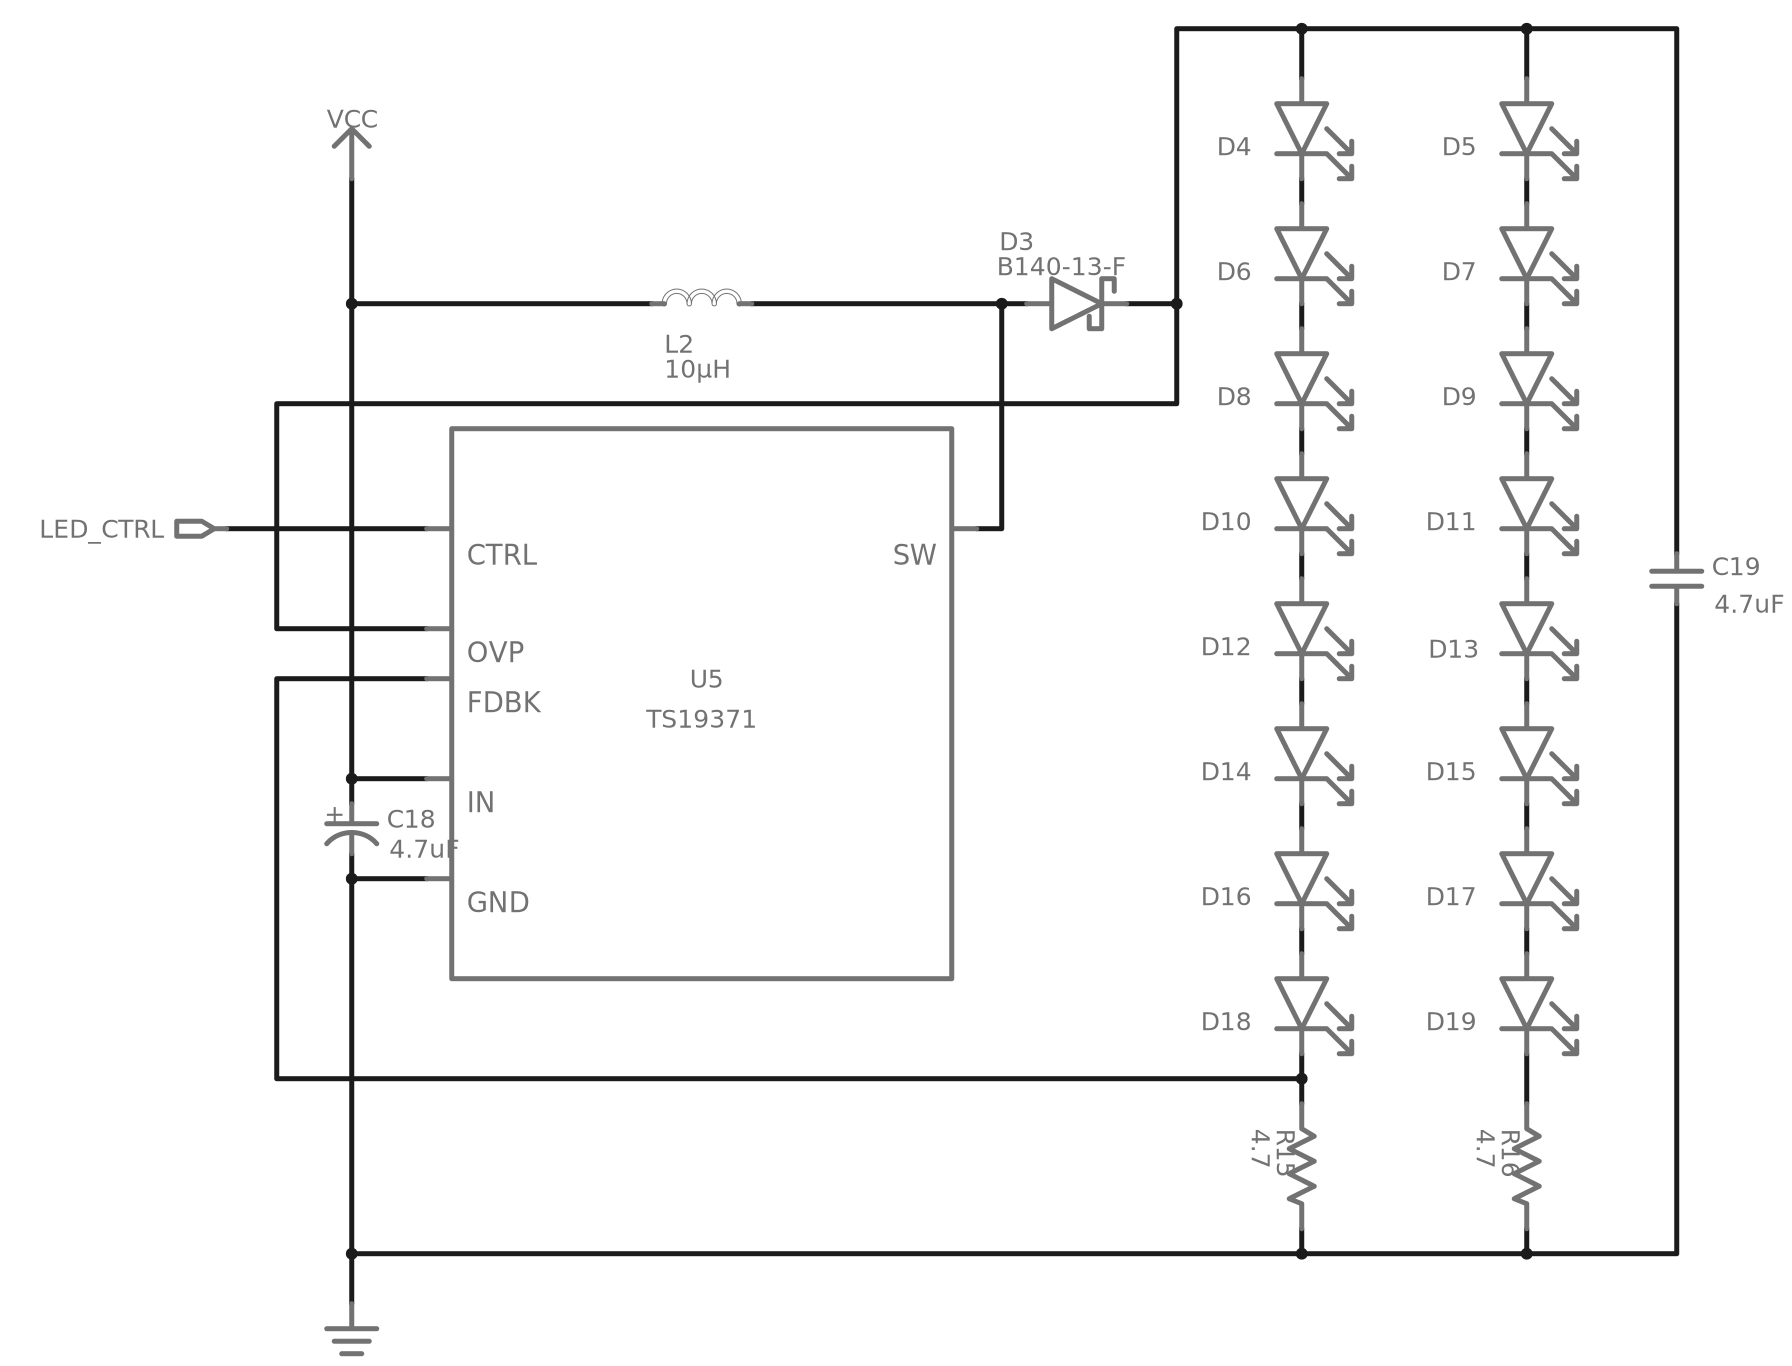
\includegraphics[width=0.85\textwidth,fbox]{img/ElecSch_LedDriver}
    }
    \caption{Schéma structurel de l'éclairage}
    \label{ElecSch_LedDriver}
\end{figure}

    La fonction électronique \emph{d'éclairage} est réalisée autour du driver de leds TS19371 (repère typographique $U_5$ de la Figure \ref{ElecSch_LedDriver}).
    Pour rappel, la fonction électronique a pour rôle d'alimenter les 16 leds blanches en fonction du signal PWM \emph{LED\_CTRL} délivré par le Raspberry Pi.
    
    Le driver de led permet de piloter deux lignes de 8 leds en série en augmentant la tension d'alimentation $VCC$ de 5V jusqu'à 18V.
    Ceci se fait en asservissant le courant sur chacune des deux lignes.
    La valeur du courant est fixée par le choix de $R_{15}$ et de $R_{16}$ :
    
\begin{equation}
R_{15} = R_{16} = \frac{95 mV}{I_{LED}} = \frac{95 mV}{20 mA} \approx 4.7 \Omega
\end{equation}

\begin{figure}[H]
    \centerline{
        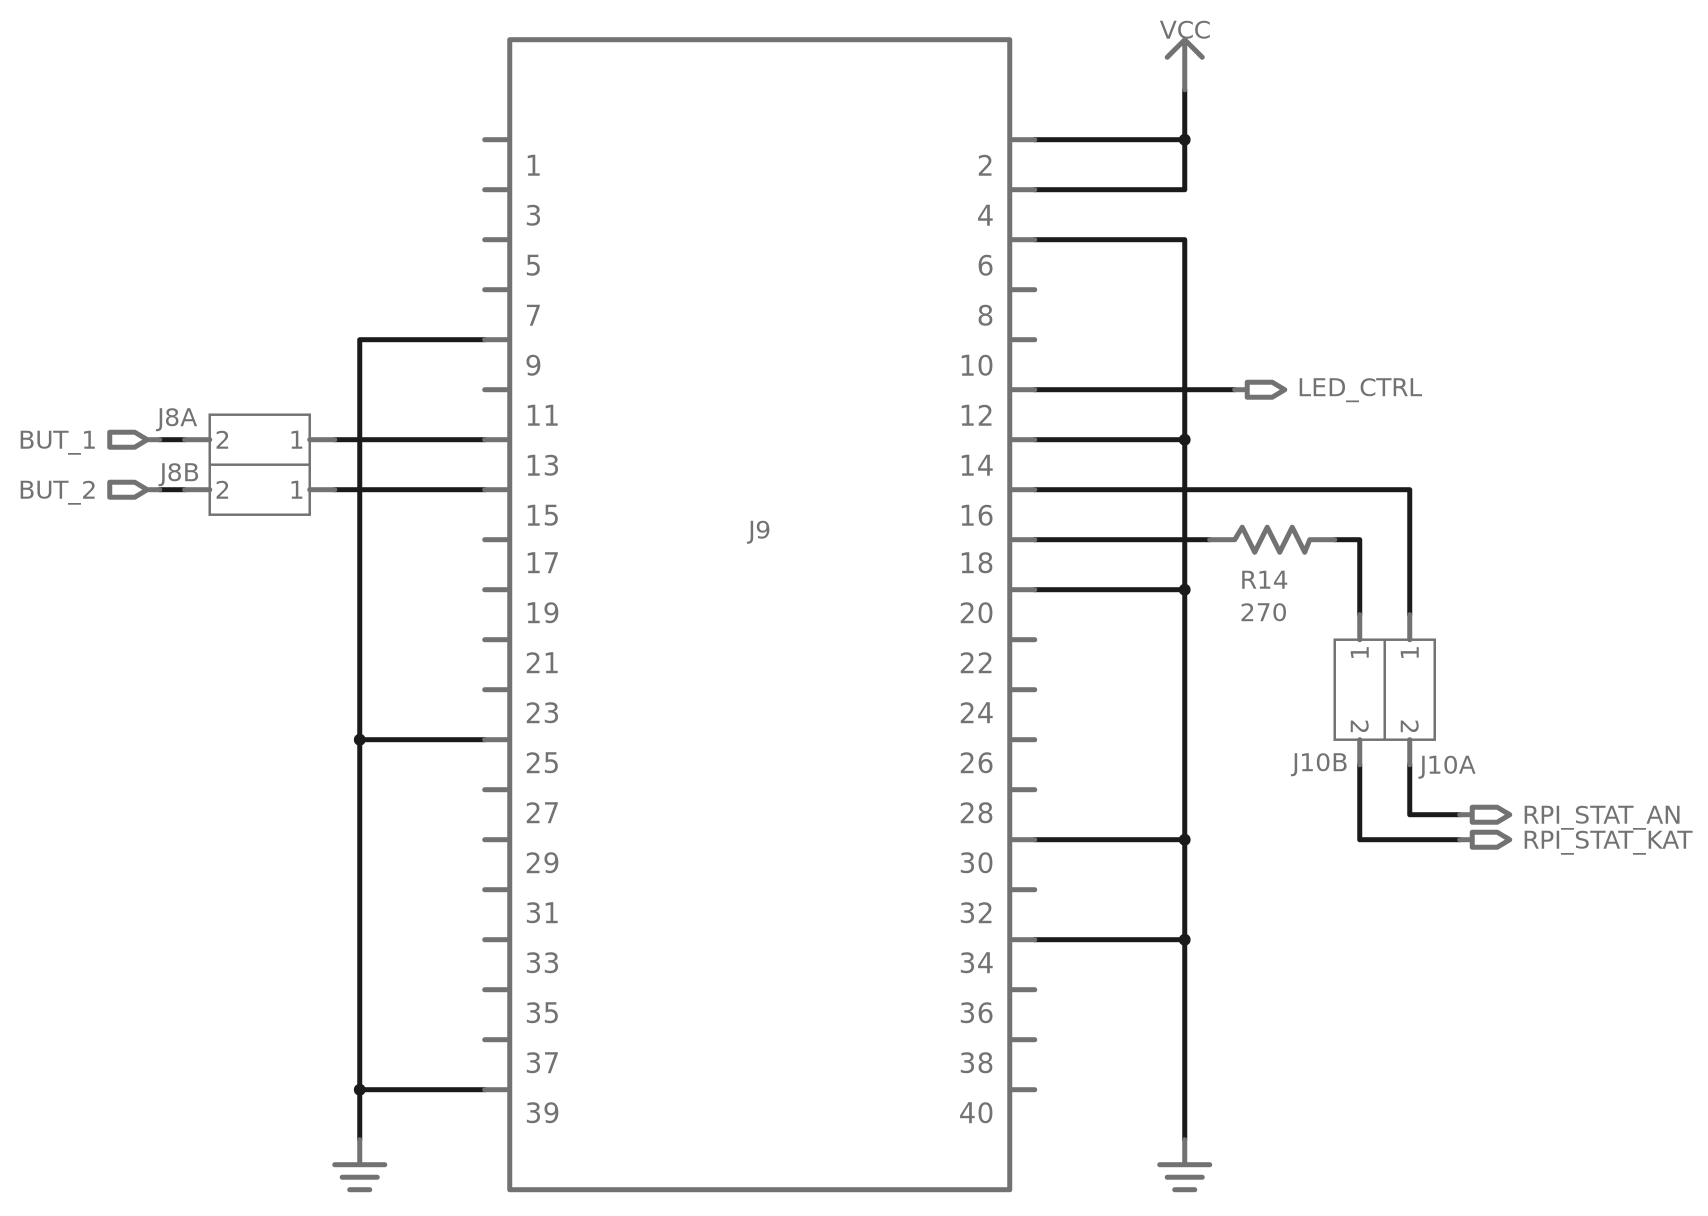
\includegraphics[width=0.85\textwidth,fbox]{img/ElecSch_RPiConn}
    }
    \caption{Schéma structurel du connecteur du Raspberry Pi}
    \label{ElecSch_RPiConn}
\end{figure}

Finalement sur la Figure \ref{ElecSch_RPiConn} on retrouve le connecteur de la Raspberry Pi sur lequel est reliée l'alimentation 5V, un premier bornier pour la lecture d'un bouton-poussoir, un second bornier pour le pilotage d'une led et enfin le signal PWM \emph{LED\_CTRL} pour le pilotage de l'éclairage.
    
    \section{Mécanique}
    % parlé fabrication boitier
    Le boitier mécanique a été modélisé sur le logiciel de CAD en ligne OnShape.
    Il est composé de trois pièces imprimées en PLA qui forment un cube d'environ 12 cm de côté.
    Un jeu de 0.2 mm a été prévu entre les pièces pour faciliter l'assemblage.
    L'assemblage final est présenté sur le dessin technique page \pageref{mecdrawing}.
    
    La première pièce constitue la trappe d'accès, elle forme une des faces du cube.
    Elle est maintenue aux deux autres pièces à l'aide de quatre vis M3 à tête conique afin d'en permettre le démontage/remontage ainsi que l'accès aux composants.
    Sur sa face sont percés les évents du haut-parleur, ce dernier est maintenu à l'aide de deux rails, ce qui permet un montage sans visserie ni colle.
    Le compartiment pour la batterie a été placé sur cette pièce.
    Les trois perçages visibles ont été placés afin d'y accueillir deux leds, l'une sert d'indicateur de charge de batterie et l'autre d'indicateur de statut du Raspberry Pi, ainsi qu'un bouton-poussoir pour lancer un scénario de reconnaissance.
    
    
    \includepdf[pages={-},angle=90]{img/Drawing_Boitier.pdf}
    \label{mecdrawing}
    
    \section{Webservices}
    
    L'ensemble des Webservices tels qu'ils sont présentés dans l'annexe A de \cite{OBCdS} ont été implémentés avec le framework Scalatra.
    L'ensemble du projet utilise le moteur de production SBT, cet outil permet de gérer notamment les dépendances de librairies, la compilation et le test.
    
    La persistance des données est faite sur une base de données dite NoSQL, MongoDB.
    L'accès à MongoDB en Scala se fait via le driver Casbah, il permet de manipuler les documents MongoDB de la même manière que l'on manipule les collections en Scala.
    Le module GridFS de MongoDB est utilisé afin d'outrepasser la limite des 16 Mo par fichier.
    
    Les services qui font appel soit à des ressources matérielles de la Raspberry Pi, soit à des tâches de calcul intensives --- comme le traitement d'image et la classification automatique --- le font en faisant des commandes système.
    Les programmes qui sont appelés ont été écrits en C++.
    
    
    % Stack scalatra + mongodb + call to external program (native c++ opencv) pico2wave => les webservices
    

\chapter{Analyse logicielle}
\label{AnaLog}
    \section{Étalonnage de caméra}
    
\begin{figure}[H]
    \centering
    \subfloat[Image originale]{
        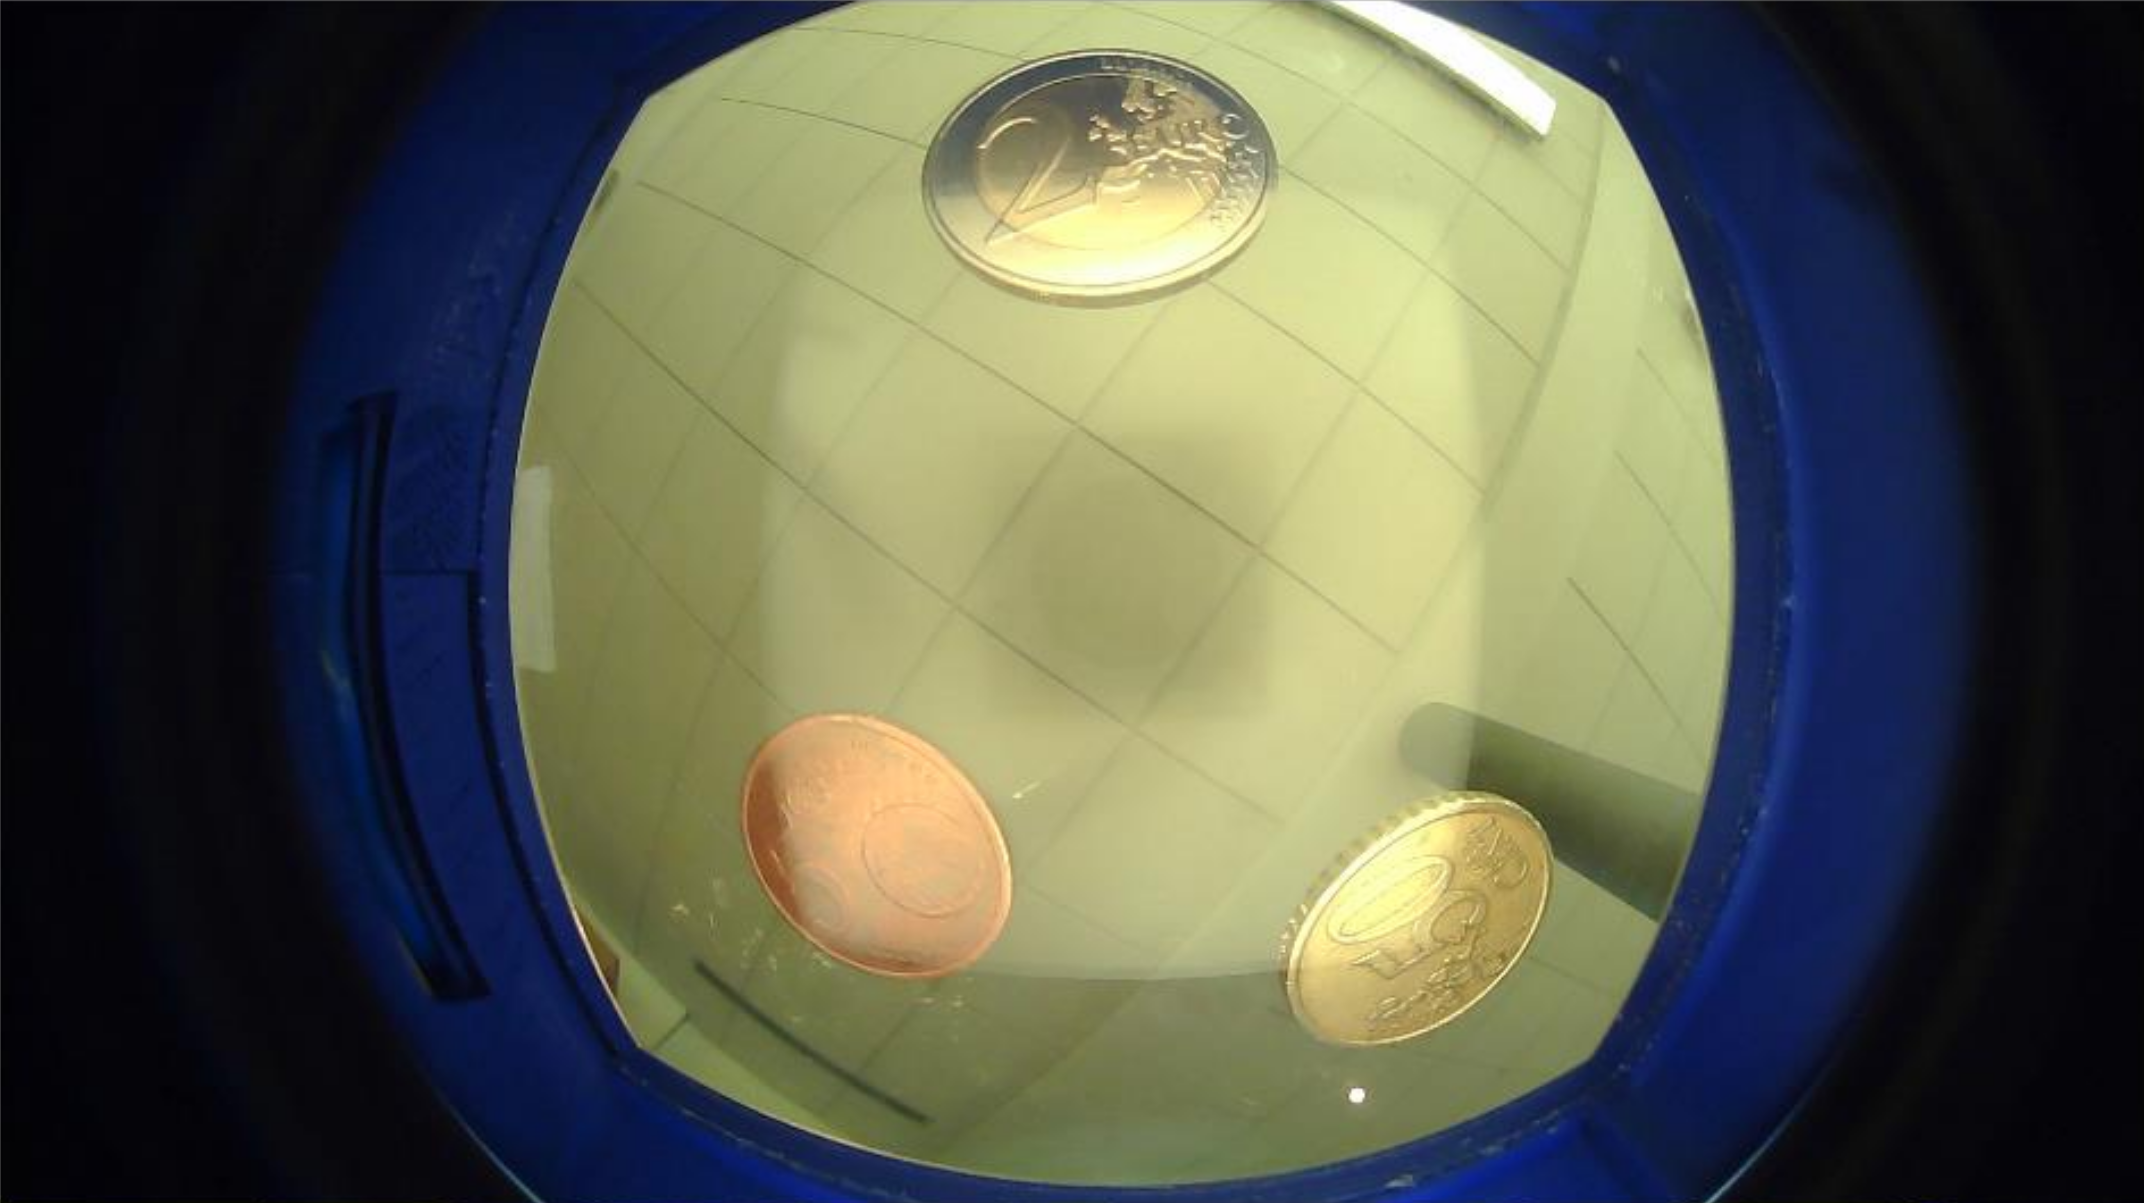
\includegraphics[width=0.6\textwidth]{img/Calibration_Original}
        \label{Calibration_Original}
    }
    \qquad
    \subfloat[Image de référence pour la calibration]{
        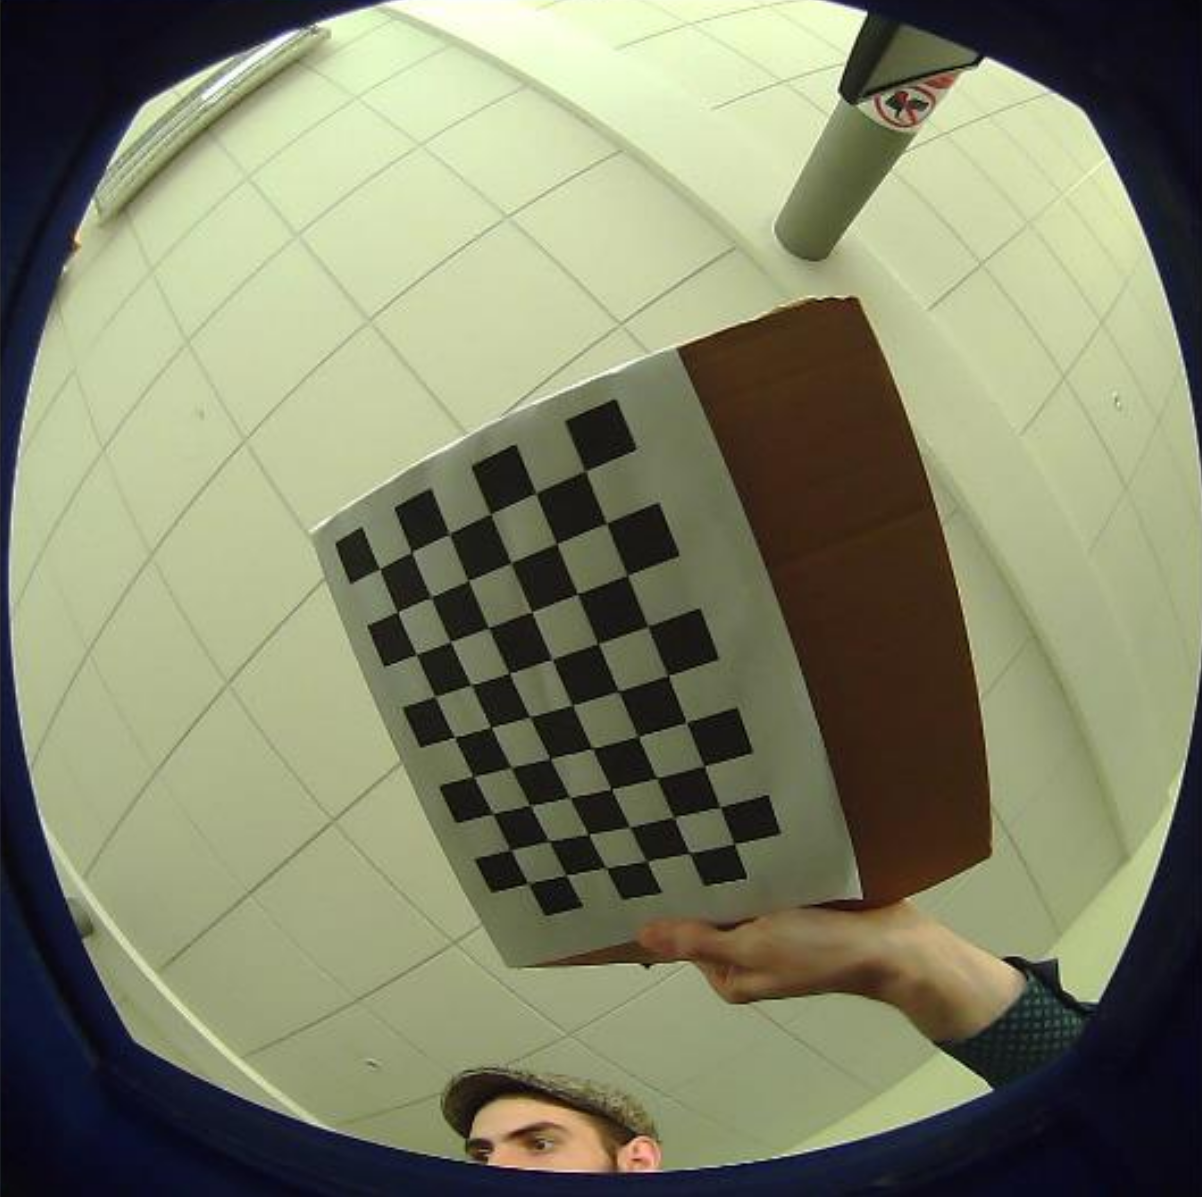
\includegraphics[width=0.4\textwidth]{img/Calibration_Chessboard}
        \label{Calibration_Chessboard}
    }
    \subfloat[Image recalibré]{
        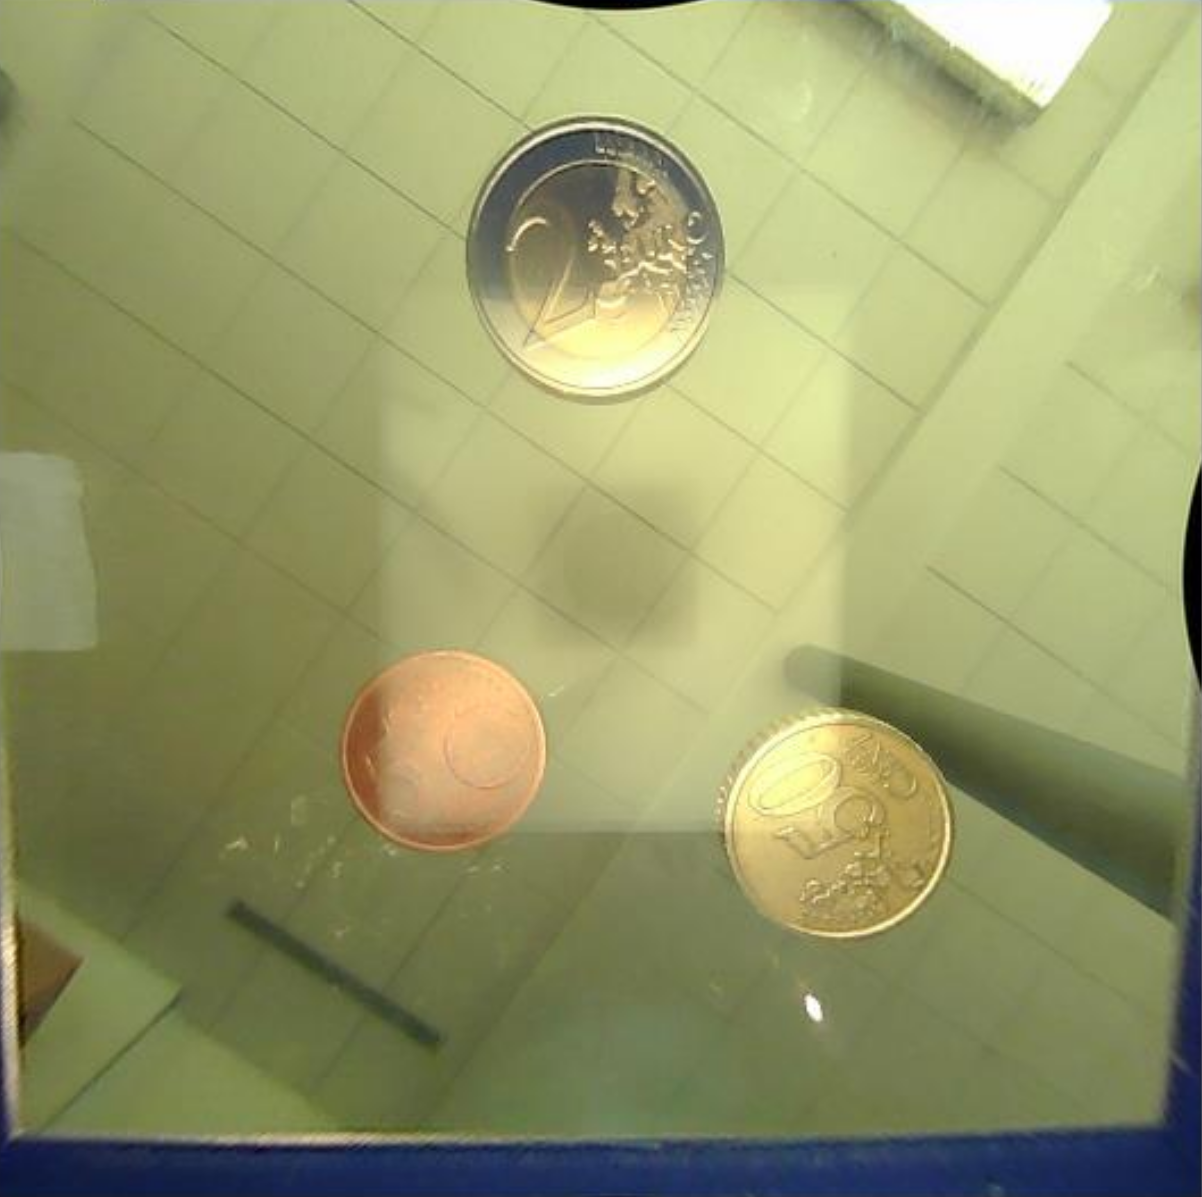
\includegraphics[width=0.4\textwidth]{img/Calibration_Undist}
        \label{Calibration_Undist}
    }
    \caption{Étalonnage de caméra}
    \label{CameraCalib}
\end{figure}

Avant l'opération de calibration de caméra, une première étape de recadrage est nécessaire.
À partir de l’image brute de 1920x1080p est faite une image carrée de 1080 pixels de côtés centrés sur la plaque.
La deuxième action est le remapage de l’image afin de corriger les problèmes de déformations géométriques causés par l’objectif.
La Figure \ref{CameraCalib} montre le résultat de cette calibration.
Pour calculer les coefficients de distorsions de la caméra, OpenCV fournit des fonctions utilitaires permettant de les calculer à partir d’un set d’images contenant un motif de géométrie connu (ici, un damier).
Le modèle du sténopé (aussi appelé modèle \emph{pin-hole}) n'est pas utilisé ici, on lui préférera le modèle dit \emph{fish-eye} ( les détails sont disponibles sur \url{http://docs.opencv.org/3.2.0/db/d58/group__calib3d__fisheye.html}).

    
    \section{Segmentation}
    
La segmentation d'image est une opération de traitement d'images qui a pour but de
rassembler des pixels entre eux suivant des critères prédéfinis.
Les pixels sont ainsi regroupés en régions, qui constituent un pavage ou une partition de l'image.
Il peut s'agir par exemple de séparer les objets du fond.

\begin{figure}[H]
    \centering
    \subfloat[Différence absolue]{
        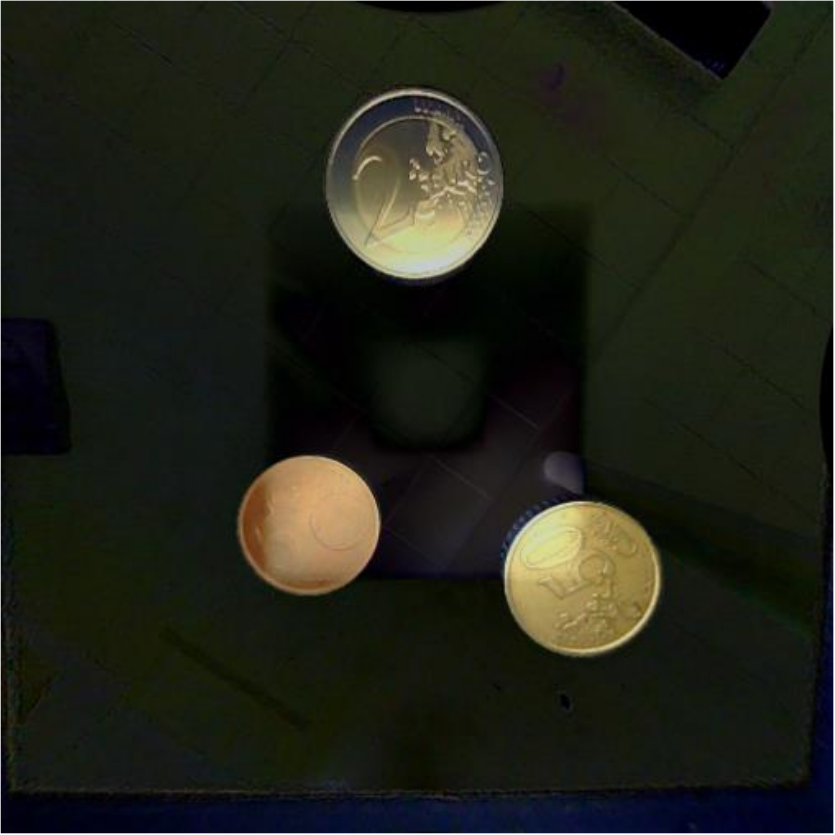
\includegraphics[width=0.3\textwidth]{img/Segmentation_AbsDiff}
        \label{Segmentation_AbsDiff}
    }
    \subfloat[Canal de teinte flouté]{
        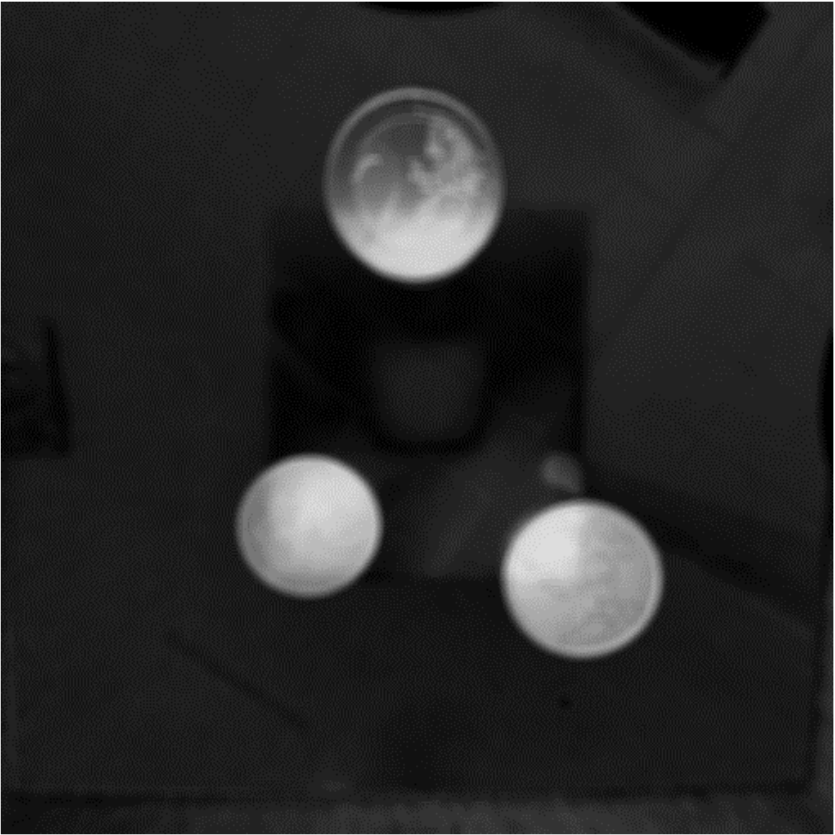
\includegraphics[width=0.3\textwidth]{img/Segmentation_HueBlurred}
        \label{Segmentation_HueBlurred}
    }
    \subfloat[Seuillage]{
        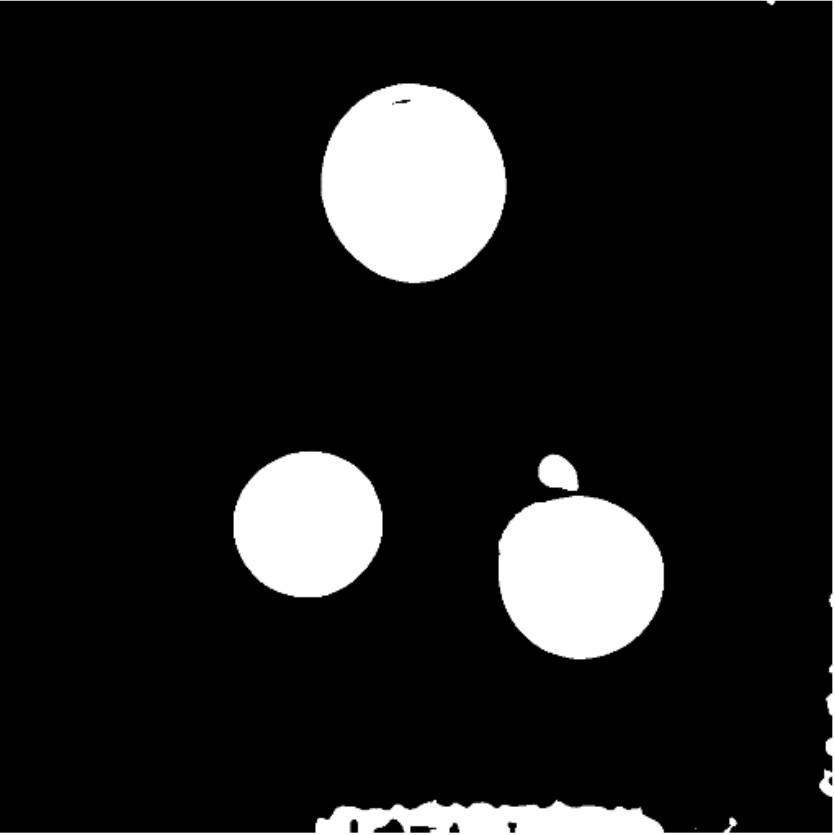
\includegraphics[width=0.3\textwidth]{img/Segmentation_Threshold}
        \label{Segmentation_Threshold}
    }
    \qquad
    \subfloat[Érosion]{
        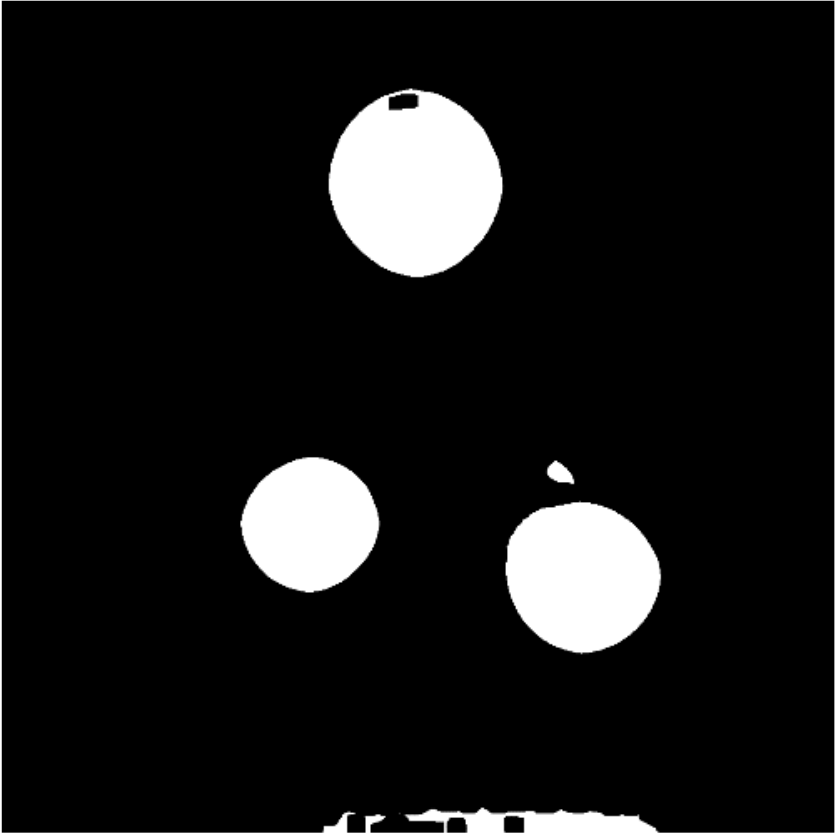
\includegraphics[width=0.3\textwidth]{img/Segmentation_Erosion}
        \label{Segmentation_Erosion}
    }
    \subfloat[Dilatation]{
        
\includegraphics[width=0.3\textwidth]{img/Segmentation_Dilatation}
        \label{Segmentation_Dilatation}
    }
    \subfloat[Rectangles circonscrit]{
        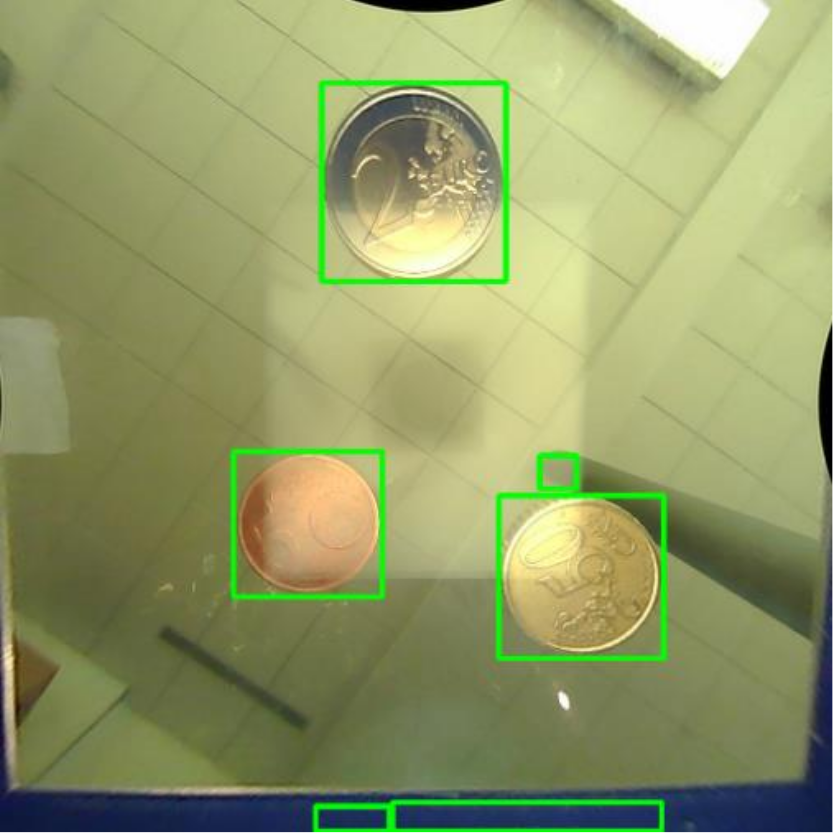
\includegraphics[width=0.3\textwidth]{img/Segmentation_BoundRect}
        \label{Segmentation_BoundRect}
    }
    \caption{Processus de segmentation}
    \label{segfig}
\end{figure}

Pour la Or-Box le pipeline de segmentation est assez simple.
Une fois les deux images obtenues, une avec éclairage et l’autre sans, on effectue les opérations suivantes :

\begin{itemize}
    \item On effectue la différence absolue des deux images, voir Figure \ref{Segmentation_AbsDiff}.
    \item On recode l’image obtenue en HSV (Hue / Saturation / Value) pour n’utiliser que le canal de valeur, car c’est dans celles-ci qu’est contenue l’information de luminosité pour chaque pixel.
    \item On floute le canal de valeur, en effectuant une convolution avec un noyau gaussien par exemple, voir Figure \ref{Segmentation_HueBlurred}.
    Cette étape n’est nécessaire que pour éviter un maximum de bruit lors de l’étape de seuillage suivante.
    \item L’étape de \emph{thresholding} (seuillage) consiste à appliquer la règle suivante pour chaque pixel :

\begin{absolutelynopagebreak}
    \begin{algorithmic}
    \If {$valeur \ge maxval$}
        \State $valeur \gets valeur_{max}$
    \Else
            \State $valeur\gets valeur_{min}$
    \EndIf
    \end{algorithmic}
\end{absolutelynopagebreak}

    Il ne reste plus qu’à trouver la valeur de seuil adapté.
    Il existe des méthodes de calcul de ce seuil basé sur les histogrammes –-- nous en avons utilisé principalement deux, soit la méthode d’Otsu \cite{otsu1975threshold} ou soit la méthode du triangle.
    
    Ces méthodes de segmentation avec un seuil globale ne marchent que si l’on suppose que l’histogramme de l’image est bimodal, c’est-à-dire qu’il existe deux piques d’intensité, un représentant les objets en premier plan et le second l’arrière-plan. Le résultat est visible sur la Figure \ref{Segmentation_Threshold}.
    \item Les opérations suivantes, l’érosion et la dilatation sont deux opérations morphologiques de base.
    Ces deux étapes servent à éliminer les régions blanches les plus petites, et à rassembler les plus proches en une seule plus grandes.
    \item La dernière étape consiste à trouver les contours des régions blanches, et trouver les rectangles circonscrits à ces contours, en vert sur la Figure \ref{Segmentation_BoundRect}.
    On effectuera ensuite le calcul des descripteurs et la classification seulement pour chacune des régions trouvées.
\end{itemize}
    
    \section{Classification automatique}
        \subsection{Définition formelle de la problématique}
        
        Formellement, le problème de la reconnaissance de forme dans un contexte d'apprentissage supervisé peut-être formulé ainsi :
        
        On considère la fonction inconnue $g:\mathcal{X}\rightarrow\mathcal{Y}$ qui définit pour chaque instance $\boldsymbol{x} \in \mathcal{X}$ en entrée, une étiquette $\boldsymbol{y} \in \mathcal{Y}$ en sortie .
        À partir des données d'entraînement $\mathbf{D} = \{(\boldsymbol{x}_1,y_1),\dots,(\boldsymbol{x}_n, y_n)\}$ que l'on considère comme étant des exemples corrects du passage entre les deux espaces, le but est de produire une fonction $h:\mathcal{X}\rightarrow\mathcal{Y}$ qui se rapproche le plus fidèlement possible de la fonction de mappage $g$.
        Le terme "le plus fidèlement possible" est défini en théorie de la décision grâce à une fonction de coût, le but alors est de minimiser cette fonction de coût durant la phase d'apprentissage.
        Dans la pratique on ne connait ni la distribution de $\mathcal{X}$ ni la fonction véritable fonction $g:\mathcal{X}\rightarrow\mathcal{Y}$.
        La seule solution est donc de collecter un grand nombre d'échantillon issu de $\mathcal{X}$ et de les étiquetés à la main avec la valeur de $\mathcal{Y}$ correcte.
        La procédure d'entraînement et de test utilisé pour la Or-Box est décrite dans la section \ref{protocoleExp}.
        
        Dans notre problème, $\boldsymbol{x}_i$ est la représentation d'une image d'un objet posé sur la vitre et $\boldsymbol{y}$ une des étiquettes parmi "un centime", "deux centimes", "cinq centimes", etc\dots
        On parle ici de "représentation d'une image" est non de l'image en entière.
        En effet, utiliser l'image brute comme ensemble $\mathcal{X}$ conduirait à une fonction $g:\mathcal{X}\rightarrow\mathcal{Y}$ extrêmement complexe à approximer.
        Il faut donc trouver un moyen intelligent de représenter l'image afin de réduire l'espace $\mathcal{X}$.
        On parle donc de descripteurs d'images (voir section  \ref{imgDescriptors}), il s'agit d'une fonction écrite par des experts du domaine qui prend l'image brute est la décrit en terme plus simple (couleurs, textures, contours, etc\dots). 
        
        \subsection{K plus proches voisins}
        
        La méthode des K plus proches voisins est une méthode d’apprentissage supervisé.
        Elle peut être utilisé dans des problèmes de classification et de régression.
        Dans les deux cas la sortie va dépendre des $k$ échantillons de la base d'apprentisage les plus proches dans l'espace de recherche.
        Dans le cas qui nous intéresse --- le problème de classification --- la sortie est l'appartenance a une classe. 
        Un object est classifié par un vote à la majorité de ses voisins, l'objet se voit assigné à la classe la plus courante parmi ces $k$ voisins.
        Le voisinage est définie par une fonction de distance, généralement une distance euclidienne ce qui sera aussi notre cas.
        
        Les perfomances d'un classificateurs peuvent parfois être améliorer en effectuant une transformation préalable sur chacune des caractéristiques.
        Deux transformation courrantes sont la \emph{standardization} et la \emph{fuzzification} \cite{peterson2009k}.
        
\begin{figure}[H]
    \centerline{
        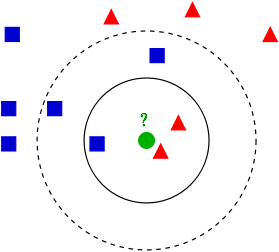
\includegraphics[width=0.35\textwidth,fbox]{img/Knn_Example}
    }
    \caption{Exemple pour classification avec K plus proches voisins - Auteur: Antti Ajanki}
    \label{KNNpic}
\end{figure}

        Dans l'exemple de la figure \ref{KNNpic}, l'échantillon à classé est représenté en vert, l'espace de recherche est à deux dimension et la base d'apprentissage contient des échantillons appartenant à deux classes, une rouge et une bleu.
        Si on choisi $k=3$ alors le cercle vert sera classé comme appartenant à la même classe que les triangles rouge, alors que pour $k=5$ il sera classé appartenant à la classe des carrés bleus.
        
        
        \subsection{Machine à vecteurs de support}
        
        Tout comme les KNN les SVM servent à résoudre des problème de classification et de régréssion.
        Cependant contrairement à ce premier ce n'est pas un algorithme \emph{lazy learning}, c'est à dire qu'il n'attend pas une requête pour essayer de généralisé les donnés d'apprentissage.
        
        Le premier problème que résout les SVM est celui de trouver une frontière séparant de manière optimale l'espace de recherche à partir de la base d'apprentissage.
        Cette frontière est un hyperplan dont la marge est maximale, c'est à dire que l'on cherche a maximiser la distance entre la frontière de séparation et les échnatillons les plus proches.
        
        Le deuxième problème que résout les SVM est celui de traiter les données qui ne sont pas linéairement séparables.
        Pour cela on cherche a paser dans un espace de plus grande dimension dans le quelle il est probable de trouver un séparation linéaire.
        Plus formellement, on applique aux vecteurs d'entrée x une transformation non-linéaire $\phi$.
        L'espace d'arrivée$\phi (X)$ est appelé espace de redescription dans lequel on peut reformuler notre recherche d'optimisation de marge.
        Cette reformulation fait apparaîtres des produits scalaires dans un espace à dimension élevée ce qui est très coûteux en terme de calcul.
        On fait alors appelà la méthode du \emph{kernel trick} qui utilise une fonction noyau pour rester dans l'espace d'origine.
        La fonction noyau doit respecter certain condition comme celle de correspondre à un produit scalaire dans un espace de grande dimension.
        
        
        \subsection{Protocole d'évaluation expérimentale}

        Chaque méthode de classification devra être testé sur l'ensemble des huit classes de pièces.
        La validité du modèle sera validé par validation croisé en \emph{"k-fold cross validation"} \cite{Refaeilzadeh2009}.
        Cette méthode consiste a diviser les échantillons originaux en $k$ sous-ensembles, puis a sélectionner l'un des $k$ sous-ensemble d'échantillons comme ensemble de validation et les ($k-1$) autres sous-ensembles constitueront l'ensemble d'apprentissage.
        On calcul l'erreur de prédiction pour l'ensemble de validation --- soit nombre d'échantillons dont la classe a été incorrectement prédit sur le nombre total d'échantillon de l'ensemble de validation.
        Puis on répète $k$ fois l'opération en sélectionnant un autre ensemble de validation parmi les ($k-1$) sous-ensembles qui n'ont pas encore été utilisés.
        Ainsi chaque échantillon a été utilisé exactement une fois comme ensemble de validation.
        L'erreur de prédiction total pour cette méthode est la moyenne des $k$ taux de prédiction.
        
        

    \section{Description d'image}
    \label{imgDescriptors}
        \subsection{Color-based descriptor}
        Une première approche pour distingué les différentes classes de pièces est de se basé sur leurs couleurs.
        Pour décrire une image par sa couleur --- ou ses couleurs --- on peut calculer son histogramme. 
        Afin de se prémunir au maximum des variations d'éclairage nous calculerons l'histogramme du canal \emph{Hue}.
        Puisque seul la distribution entre ces valeurs nous intéresse, nous les normaliserons entre 0 et 255.
        
        La figure \ref{Hists} montre les histogrammes moyens obtenues sur l'ensemble des échantillons de trois classe; la ligne bleu représente la valeur moyenne et la zone grise l'intervalle de confiance à un écart-type.
        On remarque que ces trois histogrammes sont mono-mode, que les pièces rouges ont un mode centré autour de 15, que les pièces jaunes et celles de un et deux euros ont un mode centré autour de 20.
        
\begin{figure}[H]
    \centering
    \subfloat[Pièces de un centime]{
        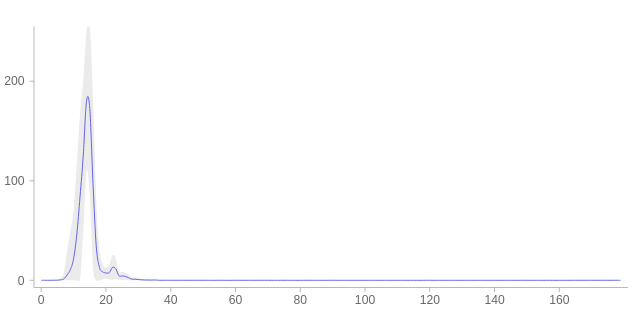
\includegraphics[width=0.6\textwidth]{img/OneCentHist}
        \label{HistOneCent}
    }
        \qquad
    \subfloat[Pièces de dix centimes]{
        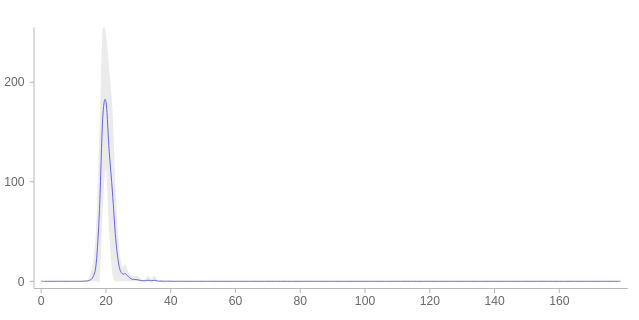
\includegraphics[width=0.6\textwidth]{img/TenCentHist}
        \label{HistTenCent}
    }
        \qquad
    \subfloat[Pièces de un euro]{
        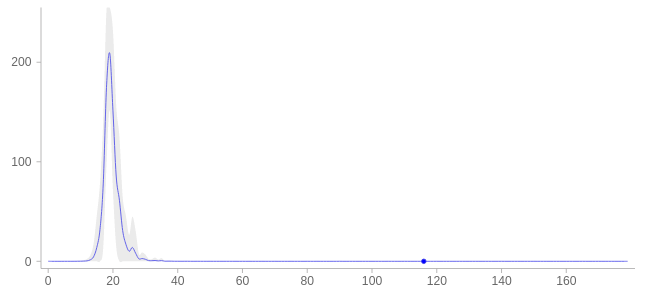
\includegraphics[width=0.6\textwidth]{img/OneEuroHist}
        \label{HistEuro}
    }
    \caption{Histogrammes moyen}
    \label{Hists}
\end{figure}
        
        \subsection{Shape-based descriptors}
        
        La distinction par couleur ne suffisant pas à distinguer les catégories entre elles, nous calculerons aussi les descripteurs suivants :
        \begin{description}
            \item[Le périmètre] du contour
            \item[L'aire]
            \item[La circularité]
            \item[Largeur du rectangle circonscrit d'aire minimum]
            \item[Hauteur du rectangle circonscrit d'aire minimum]
        \end{description}
        
        Pour chacune de ces caractéristiques ont été calculé la moyenne et l'écart-type afin de savoir si il serait potentiellement exploitable 
        
        \subsection{Binary descriptors}
        Suivant les résultats obtenues et le temps restant sur le projet des descripteurs plus complexes que ceux mentionnés ci-dessus.
        L'utilisation de ces types de descripteurs bien que très puissants et générique n'est pas une priorité pour ce projet.
        En effet, lors du projet collectif de quatrième année se sont ces méthodes qui ont était testé avec des résultats décevants --- \~30\% d'erreur.
        La faute au manque de contraste des textures visibles sur les pièces du à redéformation sur les bord de l'image.
        
 
% \nocite{*} % make all bib ref appear even if not cited
\bibliographystyle{alpha}
\bibliography{mybib}


    
        

% \begin{appendices}

\end{appendices}

\end{document}
